\documentclass[addpoints]{exam}
\usepackage{amsmath,amsthm,amssymb,url}

\usepackage{algorithm}
\usepackage{algorithmic}
\usepackage{mathtools}
\usepackage{graphicx}
\usepackage{float}
%\usepackage{tikz}
\usepackage{tkz-berge}
\usepackage[pdftex]{hyperref}
\newcommand{\abs}[1]{\left| #1\right|}

\newtheorem{lemma}{Lemma}[section]
\newcommand{\var}{\text{Var}}
\title{CS 6150: Homework 5}
\date{Due Date: December 14, 2015}
\author{Christopher Mertin\\{\scriptsize (Worked with Milinda Fernando)}}
\begin{document}
\maketitle
\begin{center}
\fbox{\fbox{\parbox{5.5in}{\centering
This assignment has \numquestions\ questions, for a total of \numpoints\
points.
Unless otherwise specified, complete and reasoned arguments will be
expected for all answers. 
}}}
\end{center}

\qformat{Question \thequestion: \thequestiontitle\dotfill \textbf{[\totalpoints]}}
\pointname{}
\bonuspointname{}
\pointformat{[\bfseries\thepoints]}

\printanswers

\begin{center}
  \gradetable
\end{center}
\newpage



\begin{questions}

\titledquestion{Integer programs}
Write down integer programs for the following problems.
\begin{parts}
  \part[10] Let $U$ be a set, and let $\mathcal{C} = \{S_1, \ldots, S_n\}$ be a
  collection of subsets of $U$. Each set $S$ has a weight $w_S$. Find a subcollection $\mathcal{C}^{\prime} \subset
\mathcal{C}$ of minimum total weight ($w(\mathcal{C}^{\prime}) = \sum_{S \in
  \mathcal{C}^{\prime}} w_S$) such that the sets in $\mathcal{C}^{\prime}$
\emph{cover} $U$: {\em i.e.}
\[ \cup_{S \in \mathcal{C}^{\prime}} S = U \]

\begin{solution}
We introduce a variable $x_{i}$ for every set $S_{i}$, such that $x_{i}=1$ if $S_{i}$ is in the set cover, and $x_{i}=0$ if it is not. The resulting function that we want to minimize is:
\begin{align}
\min\qquad & \sum_{i=1}^{n}w_{i}x_{i}\\
\text{such that:}\quad & \sum_{i:v\in S_{i}} x_{i}\geq 1\quad \forall\ v\in \mathcal{C}\\
  & x_{i}\in\{0,1\}\quad \forall\ i\in\{1,2,\ldots,n\}
\end{align}
\end{solution}


\part[10] Let $U$ be a universe, and let $\mathcal{C} = \{S_1, \ldots, S_n\}$ be a
  collection of subsets of $U$. Each element $u \in U$ has a weight $w_u$. Find
  a subset $H \subset U$ of minimum total weight ($w(H) = \sum_{u \in H} w_u$) such that each set
  in $\mathcal{C}$ is \emph{hit} by $H$: {\em i.e.}
\[ \forall S \in \mathcal{C}, H \cap S \ne \emptyset \]

\begin{solution}
To be {\em hit} by $H$, it is asking for at least one of the elements in $H$ to appear in every subset in $\mathcal{C}$. We can define a new variable $x_{i}$ for each element that is in $U$ as
\begin{align}
x_{i} &= \left\{ \begin{array} {c l} 1 & \text{choose } i^{th}\text{element of } U\\ 0 & \text{else}\end{array}\right.
\intertext{following this, we need to define a parameter $\xi_{i,\sigma}$ which represents the $\sigma^{th}$ element in $S_{i}$. This leads to the function that we want to optimize as being}
g(x) &= \min\abs{X} = \min \sum_{\sigma=1}^{\abs{U}}x_{\sigma}
\end{align}
Writing this in dual form with the constraints results in
\begin{align}
\min\qquad & \sum_{\sigma=1}^{\abs{U}}x_{\sigma}\\
\text{such that:}\quad & 
  \xi_{i,\sigma} = x_{\sigma}\\ 
& \sum_{\sigma=1}^{\abs{S_{i}}}\xi_{i,\sigma}\leq 1\quad\forall\ i\\
& x_{\sigma} > 0
\end{align}
\end{solution}

\end{parts}

\titledquestion{LP duals}
\begin{parts}
  \part[10] Consider the linear program 
  \begin{align*}
    \max\qquad & 5x + 3y - 2z \\
    \text{such that}\quad     & 3x - 2y \le 6 \\
         & 4y + 2z \le 7 \\
         & -3x + 2z \le 3
  \end{align*}
Write down the dual of this LP. 

\begin{solution}
First, we need to define our {\em dual variables} $\xi_{i}$ which to multiply all the equations. On top of which, since the original problem doesn't come with constraints on $x,\ y,\ z$, we need to bound our problem by choosing the equal to case, which gives us the (restated) problem
\begin{align}
\max\qquad & 5x + 3y - 2z\\
\text{such that}\quad & 
   \xi_{1}(3x-2y)= 6\xi_{1}\\
 & \xi_{2}(4y+2z) = 7\xi_{2}\\
 & \xi_{3}(-3x+2z) = 3\xi_{3}
\intertext{which we can simplify our constraints as being}
3x\xi_{1} - 2y\xi_{1} + 4y\xi_{2} + &2z\xi_{2} - 3x\xi_{3} + 2z\xi_{3} = 6\xi_{1}+7\xi_{2}+3\xi_{3}\\
x(3\xi_{1}-3\xi_{3})+y(-2\xi_{1}&+4\xi_{2})+z(2\xi_{2}+2\xi_{3}) = 6\xi_{1}+7\xi_{2}+3\xi_{3}
\intertext{so we want to minimize the right hand side of the above equation subject to the constraints imposed from the left hand side. This results in our equation to minimize as being}
\max\qquad &  6\xi_{1}+7\xi_{2}+3\xi_{3}\\
\text{such that}\quad & 
   3\xi_{1}-3\xi_{3}= 5\\
 & 4\xi_{2}-2\xi_{1} = 3\\
 & 2\xi_{2}+2\xi_{3} = -2\\
 & \xi_{1}, \xi_{2}, \xi_{3}\geq 0
\end{align}
\end{solution}


\part[10] Write down the dual of the linear program obtained by relaxing the
integer program from Question 1(b) above. 

\begin{solution}
This problem can be made easier by first converting the original problem into canonical form and then forming the dual from the canonical form of the problem. We can define the following variables
\begin{align}
\mathbf{x} &= \left(x_{1},x_{2},\ldots,x_{\abs{U}},\underbrace{\xi_{1,1},\xi_{1,2},\ldots,\xi_{1,\abs{S_{1}}}}_{\alpha_{1}},\ldots,\underbrace{\xi_{n,1},\xi_{n,2},\ldots,\xi_{n,\abs{S_{n}}}}_{\alpha_{n}}\right)^{T}\\
\mathbf{c} &= \left(-w_{1},-w_{2},\ldots,-w_{\abs{U}},\underbrace{0,0,0,\ldots,0}_{\beta}\right)^{T}\\
\mathbf{b} &= \left(\underbrace{-1,-1,-1,\ldots,-1}_{n},\ldots,\underbrace{0,0,0,\ldots,0}_{\gamma}\right)^{T}
\intertext{where $\alpha_{i}$ denotes which set they belong to, for example $\alpha_{1}$ is defining the indices that come from $S_{1}$. $\beta$ defines the zeros in $S_{1}+S_{2}+\cdots+S_{n}$, and $\gamma$ represents $\forall \sigma \in U \times$ the number of sets contained $\sigma$ times. From our constraints in the problem, we can build a matrix $\mathbf{A}$ as}
\mathbf{A} &= \left[ \begin{array}{c c c c c c c c c} 
0      & 0      & 0      & \cdots & 1      & 1      & \cdots & 0      & 1\\
\vdots & \vdots & \vdots & \ddots & \vdots & \vdots & \ddots & \vdots & \vdots\\
0      & 0      & 0      & \cdots & 0      & 1      & \cdots & 1      & 0\\
1      & 0      & 0      & \cdots & \Delta_{1,1,1} & 1     & \cdots & 0 & 1\\
-1     & 0      & 0      & \cdots & \Delta_{1,1,2} & 0 & \cdots & 1      & 0\\ 
\vdots & \vdots & \vdots & \ddots & \vdots & \vdots & \ddots & \vdots & \vdots\\
0      & 0      & 1      & \cdots & \Delta_{\abs{U},n,1} & 0 & \cdots & 1      & 0\\
0      & -1     & 0      & \cdots & \Delta_{\abs{U},n,2} & 1 & \cdots & 0      & 0
\end{array}\right]
\end{align}
where $\Delta_{i,j,1}$ represents the row such that there are some columns that get $1$ entries if $x_{i}\in S_{j}$, and $\Delta_{i,j,2}$ represents the row such that there are some columns that get $-1$ entries if $x_{i}\in S_{j}$. This goes down to the condition of $x_{\abs{U}}\in S_{n}$. Using these matricies and vectors, we can write the primal of the linear problem as
\begin{align}
\max\qquad &  \mathbf{c}^{T}\mathbf{x}\\
\text{such that}\quad & 
   \mathbf{A}\mathbf{x} \leq \mathbf{b}\\
 & \mathbf{x}\geq 0
\intertext{which is trivial to solve the dual of as it comes from the definition of the dual, resulting in}
\min\qquad &  \mathbf{y}^{T}\mathbf{b}\\
\text{such that}\quad & 
   \mathbf{y}^{T}\mathbf{A}\geq \mathbf{c}^{T}\\
 & \mathbf{y}\geq 0
\intertext{where}
& \mathbf{y} = \left(y_{1},y_{2},\ldots,y_{\abs{\mathbf{b}}}\right)^{T}
\end{align}
\end{solution}

\end{parts}

\titledquestion{Max cardinality matching}
\begin{parts}
  \part[10] Write down a linear program for computing a maximum cardinality
  matching in a bipartite graph. Your linear program will have one variable for
  each edge. 

\begin{solution}
We need to define a new variable that is built from the graph $G(V,E)$. We denote this variable as $\Gamma_{u,v}$ which is 1 if the edge $(u,v)$ is the one we picked to be in the perfect matching set. Since this is a bipartite graph, $u\neq v$ in any situation, so $\Gamma_{i,i} = 0$. The resulting linear program is represented as
\begin{align}
\max\qquad &  \sum_{u,v}\Gamma_{u,v}\\
\text{such that}\quad & 
   \Gamma_{u,v} + \Gamma_{u,i} \leq 1\\
&   \Gamma_{u,v} \geq 0\ \quad\forall\ u,v\\
& u\neq v\neq i\quad\forall\ u,v,i
\end{align}
\end{solution}


\part[10] Write down the dual of this LP. What well known problem does it capture? 

\begin{solution}
To write the dual of the above solution, we can first convert it into canonical form to make the process easier. We can use the following bipartite graph as a reference to building it into canonical form, where we are also assuming that the previous solution was built around this graph as well
\begin{center}
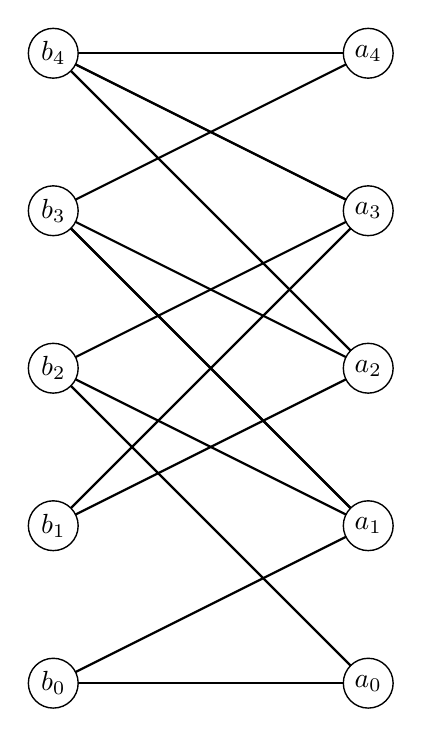
\begin{tikzpicture}
   \begin{scope}[rotate=90]
       \SetVertexMath
       \grEmptyLadder[RA=2,RB=4]{5}   
   \end{scope}
    \Edges(b2,a0,b0,a1,b2,a3,b1,a2,b3,a1,b3,a4,b4,a3,b4,a2)
\end{tikzpicture} 
\end{center}

In the primal linear program, we have $\abs{E}$ variables. To classify the number of constraints required, we need a few more definitions.

\begin{align}
\intertext{First, we make the assumption that $u_{i}\in \{B\}\ \forall\ i$ and $v_{j}\in \{A\}\ \forall\ j$, where $u_{i}$ represents the $i^{th}$ vertex in $\{B\}$ and $v_{j}$ represents the $j^{th}$ vertex in $\{A\}$. Following this, the number of constraints in the primal can be defined as} 
\Omega &= \sum_{i=1}^{\abs{B}}{\text{deg}(u_{i})\choose 2}
\intertext{which comes from the fact that we can choose edges which have the common vertex $u_{i}$. Since we have $\Omega$ constraints in the primal, we have $\Omega$ variables in the dual, which can be defined as}
\boldsymbol{\xi} &= \left(\xi_{1},\xi_{2},\ldots,\xi_{\Omega}\right)^{T}\\
\mathbf{c} &= \left(1,1,1,\ldots,1\right)^{T}\\
\mathbf{b} &= \left(1,1,1,\ldots,1\right)^{T}
\intertext{where $\boldsymbol{\xi}\in\mathbb{R}^{\Omega\times 1}$ is our vector of dual variables, and $\mathbf{c}\in\mathbb{R}^{\abs{E}\times 1}$ and $\mathbf{b}\in\mathbb{R}^{\Omega\times 1}$ come from the primal. We can build a matrix $\mathbf{M}$ which the rows represent nodes in $\{B\}$ and the columns represent nodes in $\{A\}$. This gives us}
\mathbf{M} &= \left[\begin{array}{c c c c c c c c}
1      & 1      & 1      & 0      & \cdots & 0      & 1      & 0\\
0      & 1      & 0      & 1      & \cdots & 1      & 1      & 0\\
\vdots & \vdots & \vdots & \vdots & \ddots & \vdots & \vdots & \vdots\\
1      & 0      & 0      & 1      & \cdots & 0      & 1      & 1\\
\vdots & \vdots & \vdots & \vdots & \ddots & \vdots & \vdots & \vdots\\
0      & 1      & 1      & 0      & \cdots & 0      & 0      & 1\\
\end{array} \right]
\end{align}
\begin{align}
\intertext{Now that we have all the information of the graph, we can build the linear program into canonical form}
\max\qquad &  \mathbf{c}^{T}\mathbf{x}\\
\text{such that}\quad & 
   \mathbf{M}\mathbf{x} \leq \mathbf{b}\\
 & \mathbf{x}\geq 0
\intertext{which is trivial to turn into a dual, resulting in}
\min\qquad &  \boldsymbol{\xi}^{T}\mathbf{b}\\
\text{such that}\quad & 
   \boldsymbol{\xi}^{T}\mathbf{M} \leq \mathbf{c}^{T}\\
 & \boldsymbol{\xi}\geq 0
\end{align}
The above dual finds the minimum path length to visit each node onces, so it is representative of the Traveling Salesman Problem.
\end{solution}

\end{parts}


\titledquestion{Generalized Duals}[20]

We've seen that any linear program can be written in the canonical form 
\begin{align*}
  \max \qquad & c^\top x \\
  \text{such that} \quad & Ax \le b \\
  & x \ge 0
\end{align*}

which gives rise to the corresponding dual
\begin{align*}
  \min \qquad & y^\top b \\
  \text{such that} \quad & y^\top A \ge c \\
  & y \ge 0
\end{align*}
It turns out that first transforming a general linear program with equality and
$\ge$ constraints into canonical form, and then writing the dual, can be a
little inconvenient, and that it's easier to write the dual directly. 

But what would this dual look like? Let's take a general linear program that
looks like this: 

\begin{align*}
\max \qquad & ax + by + cz \\
\text{such that} \quad & Ax + By + Cz \le d \\
& Dx + Ey + Fz = e \\
& Gx + Hy + Iz \ge f \\
& x \ge 0, z \le 0
\end{align*}

Note that $x, y, z$ are \emph{vectors} and $y$ is unconstrained (i.e the
coordinates of $y$ could be more or less than zero). 

Write down the dual of this linear program. You will do this by first
transforming this into the canonical setting, writing the canonical dual, and
then rewriting the dual in simplified form. It will help to remember that if $a$
and $b$ are two variables that are both greater than zero, then $a-b$ represents
a variable that could be either more or less than zero. 

Do you notice any pattern in the relation between primal constraint and dual
variables (and vice versa)? 

\begin{solution}
We need to define new variables $\xi_{1},\ \xi_{2},\ k$ such that $\xi_{1},\ \xi_{2},\ k \geq 0$. We also need to define $y=\xi_{1}-\xi_{2}$ and $k=-z$. Using these definitions, we can rewrite the given function as
\begin{align}
\max ax &+ by + cz\\
\max ax &+ b(\xi_{1}-\xi_{2})+c(-k)\\
\max ax &+ b\xi_{1}-b\xi_{2}-ck
\end{align}
\begin{align}
\intertext{we can do the same thing as above to our constraints, which will then be rewritten as}
Ax + B\xi_{1}-B\xi_{2}-Ck &\leq d\\
Dx + E\xi_{1}-E\xi_{2}-Fk &\leq e\label{eq:equal1}\\
-Dx- E\xi_{1}+E\xi_{2}+Fk &\leq -e\label{eq:equal2}\\
-Gx-H\xi_{1}+H\xi_{2}+Ik &\leq -f
\end{align}
\begin{align}
\intertext{where Equation (\ref{eq:equal2}) is just the negative of Equation (\ref{eq:equal1}) which comes about due to the equal sign on the given constraints (we need to check both limits). Following this, we can define}
\mathbf{x} &= \left(x,\xi_{1},\xi_{2},k\right)^{T}\\
\mathbf{M} &= \left[ \begin{array}{r r r r} A & B & -B & -C\\D & E & -E & -F\\-D & -E & E & F\\-G & -H & H & I\\\end{array}\right]\\
\mathbf{b} &= \left(d,e,-e,-f\right)^{T}\\
\boldsymbol{\xi} &= \left(\xi_{1},\xi_{2},\xi_{3},\xi_{4}\right)^{T}
\end{align}
\begin{align}
\intertext{where we can write the dual of the original problem as being}
\max\qquad & \mathbf{c}^{T}\mathbf{x}\\
\text{such that}\quad & \mathbf{M}\mathbf{x}\leq \mathbf{b}\\
& \mathbf{x}\geq 0
\intertext{where the dual of this is}
\min\qquad & \boldsymbol{\xi}^{T}\mathbf{b}\\
\text{such that}\quad & \boldsymbol{\xi}^{T}\mathbf{M}\geq \mathbf{c}\\
& \boldsymbol{\xi} \geq 0
\intertext{which can be simplified to}
\min\qquad & d\xi_{1}+e\xi_{2}-e\xi_{3}-f\xi_{4}\\
\text{such that}\quad & A\xi_{1} + D\xi_{2}-E\xi_{3}-H\xi_{4}\geq a\\
& B\xi_{1}+E\xi_{2}-E\xi_{3}-H\xi_{4}\geq b\\
& -B\xi_{1} - E\xi_{2} + E\xi_{3}+H\xi_{4}\geq -b\\
&-C\xi_{1}-F\xi_{2}+F\xi_{3}+I\xi_{4}\geq -c\\
&\boldsymbol{\xi}\geq 0
\end{align}
{\bf Patterns}:
\begin{itemize}
\item The dual of a given primal is the opposite. For example, if the primal is a maximization problem, then the dual will be a minimization problem.
\item The number of variables in one linear program corresponds to the opposite's number of constraints. For example, if a given primal has $m$ variables, then the corresponding dual has $m$ constraints. And if a dual has $n$ variables, it corresponds to $n$ constraints in the primal.
\item When converting the primal into canonical form, we need to introduce dual variables, for which in this case we introduced $\xi_{1},\ \xi_{2}$. In the dual, we had the equality constraint $B\xi_{1}+E\xi_{2}-E\xi_{3}-H\xi_{4}=b$, where $b$ was multiplied by $(\xi_{1}-\xi_{2})$ in the beginning, thus the equality constraint came from the constant that was first multiplied by the dual variables in the original linear program.
\end{itemize}
\end{solution}


\titledquestion{Best fit line}[20]
\emph{this is question 7(b) from the Erickson notes on LPs}

You are given $n$ points $(x_i, y_i)$ in the plane, and you wish to find a line
of \emph{best fit}. But instead of the standard squared error norm, you will be
using the $\ell_1$ error: namely, for any given line $y = ax + b$, the error is
given by 
\[ \epsilon_1(a, b) = \sum_{i=1}^n |y_i - (ax_i + b)|. \]
Write down a linear program to find a line that minimizes $\epsilon_1$. 

\begin{solution}
In order to minimize the function, we want to minize the following
\begin{align}
\min_{x}\qquad & \sum_{i=1}^{n}\left| a_{i}^{T}x_{i}-b_{i}\right|\\
\intertext{To get into linear programming form, we need a bound on the variables. Since the data can be on {\em either side} of the line in question, we need to take that into account when building the bounds. First, we define a variable $\xi_{i}=y_{i}-(ax_{i}+b)$, which will help in bounding the problem. It represents how close our line of best fit is to the data point. This results in the following minimization problem}
\min_{x,\xi}\qquad & \sum_{i=1}^{n}\xi_{i}\\
\text{such that:}\quad & -\xi_{i}\leq y_{i}-a_{i}x_{i}-b_{i}\leq \xi_{i}\qquad \forall\ i\in\{1,2,\ldots,n\}
\end{align}
\end{solution}



\end{questions}

\end{document}

%%% Local Variables:
%%% mode: latex
%%% TeX-master: t
%%% End:
